\documentclass[border=10pt]{standalone}
\usepackage{tikz}\usepackage{amsmath}\usetikzlibrary{arrows.meta}
\begin{document}
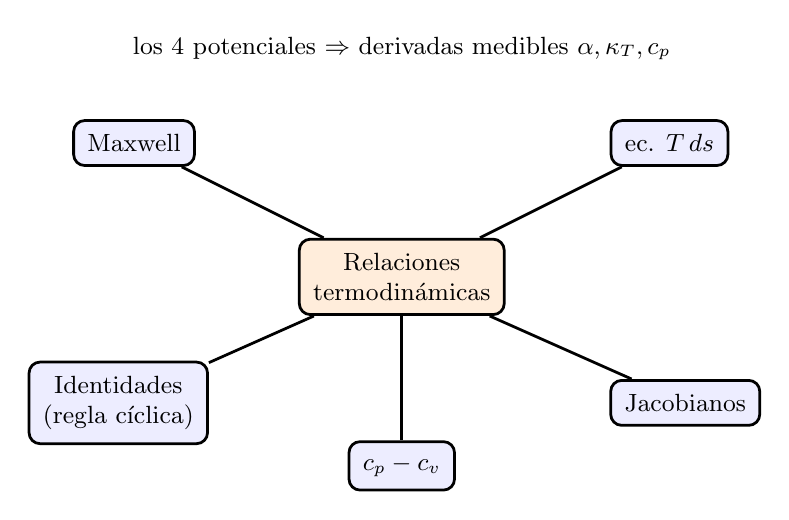
\begin{tikzpicture}[font=\small,
  nd/.style={draw,line width=1pt,rounded corners,fill=blue!7,align=center,inner sep=5pt}]
  \node[nd,fill=orange!14] (c) at (0,0) {Relaciones\\termodinámicas};
  \node[nd] (mx) at (-3.4,1.7) {Maxwell};
  \node[nd] (td) at (3.4,1.7) {ec. $T\,ds$};
  \node[nd] (id) at (-3.6,-1.6) {Identidades\\(regla cíclica)};
  \node[nd] (cc) at (0,-2.4) {$c_p-c_v$};
  \node[nd] (jc) at (3.6,-1.6) {Jacobianos};
  \foreach \n in {mx,td,id,cc,jc} \draw[line width=1pt] (c)--(\n);
  \node at (0,2.9){los 4 potenciales $\Rightarrow$ derivadas medibles $\alpha,\kappa_T,c_p$};
\end{tikzpicture}
\end{document}
